
\documentclass[11pt,a4paper,computermodern]{article}


\usepackage[
%	includeheadfoot,
	width=172mm,
	top=18mm,
	bottom=18mm,
	bindingoffset=4mm
	]{geometry}


%%% Typeface packages
\usepackage[utf8]{inputenc}
\usepackage[T1]{fontenc}
\usepackage{fontawesome}

\usepackage{multirow}
\usepackage{tabularx}
\usepackage{booktabs}
\usepackage[flushleft]{threeparttable}
\usepackage{enumitem}

%%% Graphics packages
\usepackage{graphicx}

%%
\usepackage{hyperref}
\hypersetup{
	colorlinks=false,
	hidelinks=true,
}


%%
\newcommand{\code}{\texttt}

%%
\title{Stripe Data Architecture}
\date{}


\begin{document}

\maketitle

\vspace{-10mm}

Stripe is a leading global financial technology company, founded in 2010, that powers online payment processing for millions of businesses across over 120 countries. With billions of transactions processed annually and clients ranging from startups to Fortune 500 companies, Stripe operates at massive scale and complexity. As its operations have grown, Stripe's data architecture has become a strategic priority, requiring the integration in a single system of a large variety of data. This proposal outlines a comprehensive data infrastructure designed to ensure performance, consistency, and compliance while enabling advanced use cases such as fraud detection, customer insights, and predictive analytics.


\section*{Architecture Overview}

The data integration architecture is presented in figure~\ref{fig:architecture}. It follows a hybrid model combining real-time streaming and batch processing, supporting low-latency data sync for operational use cases (e.g., fraud detection) and high-throughput batch processing for analytics.
\begin{itemize}[itemsep=5pt, parsep=0pt]
	\item Data streams originating from Stripe API (e.g. bank transaction information, telemetry) are pipelined to the relevant database systems using kafka streams.
	\item A reference database holds slowly changing reference data such as country and currency codes, merchant information of currency exchange rates. Any change in this data is reflected to the systems that depend on it through change data capture (CDC).
	\item Data is archived periodically in a data lake, with batch processing managed by Apache Airflow.
	\item The loading of less time-sensitive data such as audit logs or customer feedback is handled by Airflow batches.
\end{itemize}


\begin{figure}[h]
	\centering
	\includegraphics[scale=0.93]{./figures/architecture}
	\caption{Overview of the proposed data architecture. The description is given in the text. The lock symbols in the OLTP and Reference databases indicate that the security of these systems is critical.}
	\label{fig:architecture}
\end{figure}


We present in table~\ref{table:providers} a list of possible providers for the various systems of our architecture.

\begin{table}[ht]
	\centering
	\begin{threeparttable}
		\caption{Proposed providers for the various systems of the architecture.}
		\label{table:providers}
		\begin{tabularx}{0.99\textwidth}{c >{\centering\arraybackslash}X}
			\toprule
			System & Provider  \\
			\midrule
			OLTP/OLAP & Snowflake, Redshift \\
			NoSQL & MongoDB, DynamoDB \\
			Data Lake & Amazon S3, Azure Data Lake \\
			\bottomrule
		\end{tabularx}
	\end{threeparttable}
\end{table}

\section*{Reference Database}

Slowly changing or static reference data (e.g. country reference, merchant information, currency change rates) is stored in a reference database that serves as a single source of truth. The OLTP, OLAP and NoSQL systems incorporate a copy of the relevant reference tables for faster access. Central updates are propagated through change data capture (CDC). The data is subject to the security and compliance policy described below (e.g. encryption of merchant information). This approach has the advantage of a finer-grained monitoring and control of data access and modification. We present in table~~\ref{table:ReferenceDataDict} a data dictionary for some tables in the reference database.

\begin{table}[ht]
	\centering
	\begin{threeparttable}
		\caption{Data dictionary for the \code{transactions} OLTP schema.}
		\label{table:ReferenceDataDict}
		\begin{tabularx}{0.99\textwidth}{c c >{\centering\arraybackslash}X >{\centering\arraybackslash}X}
			\toprule
			Field Name & Type & Description & Example  \\
			\midrule
			\multicolumn{4}{c}{\code{countries} table}\\
			\code{country\_code} & \code{char(2)} & ISO 3166-1 2-letter & \code{'GB'} \\
			\code{country\_name} & \code{text} & Country name & \code{'United Kingdom'} \\
			
			\midrule
			\multicolumn{4}{c}{\code{currencies} table}\\
			\code{currency\_code} & \code{char(3)} & Currency code (ISO 4217) & \code{'EUR'} \\
			\code{currency\_name} & \code{text} & Currency name & \code{'Euro'} \\
			\code{usd\_change\_rate} & \code{char(2)} & Currency to USD change rate & \code{1.08} \\
			
			\midrule
			\multicolumn{4}{c}{\code{merchants} table}\\
			\code{merchant\_id} & \code{bigint} & Unique merchant id & \code{12345} \\
			\code{name} & \code{text} & Merchant name & \code{'Amazon UK'} \\
			\code{iban} & \code{text} & Merchant IBAN & \code{'GB82WEST12345678765432'} \\
			\code{country\_code} & \code{char(2)} & Merchant registration country & \code{'GB'} \\
			
			\midrule
			\multicolumn{4}{c}{\code{customers} table}\\
			\code{customer\_id} & \code{bigint} & Unique customer id & \code{234567} \\
			\code{name} & \code{text} & Customer name & \code{'John Doe'} \\
			\code{iban} & \code{text} & Customer IBAN & \code{'GB82WEST12345678765432'} \\
			\code{country\_code} & \code{char(2)} & Customer country code  & \code{'GB'} \\
			
			\bottomrule
		\end{tabularx}
	\end{threeparttable}
\end{table}


\section*{Online Transaction Processing (OLTP) Data Model}

Our proposed OLTP database architecture is presented in figure~\ref{fig:OLTP}. The core of the database is a registry of all financial transactions occurring within Stripe scope. Tables containing information about merchants and customers are cached from the reference database. Fraud indicators are stored in a dedicated table in a one-to-one correspondence with the main transactions table. The rationale behind this choice is that fraud indicators originate from a different pipeline (e.g. reports after bank investigation).


\begin{figure}
	\centering
	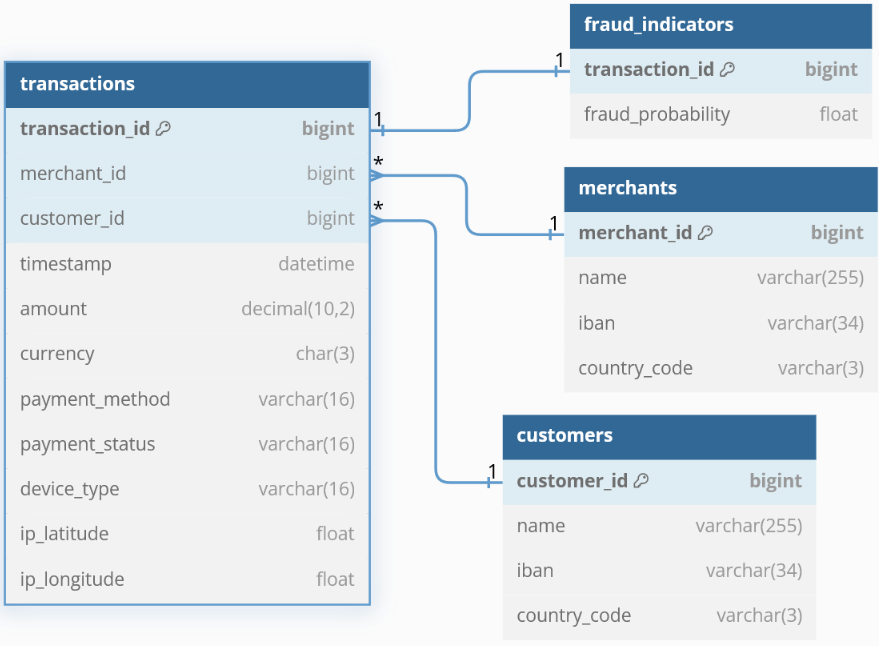
\includegraphics[scale=0.7]{./figures/OLTP}
	\caption{Proposed OLTP database structure.}
	\label{fig:OLTP}
\end{figure}


\begin{table}[ht]
	\centering
	\begin{threeparttable}
		\caption{Data dictionary for the \code{transactions} OLTP schema.}
		\label{table:OLTP}
		\begin{tabularx}{0.99\textwidth}{c c >{\centering\arraybackslash}X >{\centering\arraybackslash}X}
			\toprule
			Field Name & Type & Description & Example  \\
			\midrule
			\multicolumn{4}{c}{\code{transactions} table}\\
			\code{transaction\_id} & \code{bigint} & Unique transaction id & \code{123456789} \\
			\code{merchant\_id} & \code{bigint} & Merchant id & \code{12345} \\
			\code{customer\_id} & \code{bigint} & Customer id & \code{234567} \\
			\code{timestamp} & \code{datetime} & UTC transaction timestamp & \code{2023-11-18T17:43:02.4} \\
			\code{amount} & \code{float} & Transaction amount & \code{43.15} \\
			\code{fee} & \code{float} & Transaction fee & \code{0.53} \\
			\code{currency\_code} & \code{char(3)} & Currency code (ISO 4217) & \code{'GBP'} \\
			\code{payment\_method} & \code{text} & Payment method & \code{'credit\_card'} \\
			\code{payment\_status} & \code{text} & Transaction status & \code{'sucess'} \\
			\code{device\_type} & \code{text} & Device used for payment & \code{'mobile'} \\
			\code{ip\_latitude} & \code{float} & IP-based geolocation latitude & \code{49.6833300} \\
			\code{ip\_longitude} & \code{float} & IP-based geolocation longitude & \code{10.5333300} \\
			
			\midrule
			\multicolumn{4}{c}{\code{fraud\_indicators} table}\\
			\code{transaction\_id} & \code{bigint} & Transaction id & \code{123456789} \\
			\code{is\_fraud} & \code{boolean} & Is the transaction a fraud ? & \code{false} \\
			\bottomrule
		\end{tabularx}
	\end{threeparttable}
\end{table}


\section*{Online Analytical Processing (OLAP) Data Model}

Pour l'analyse et la préparation de features pour la détection de fraude, on utilisera une base 


\begin{figure}
	\centering
	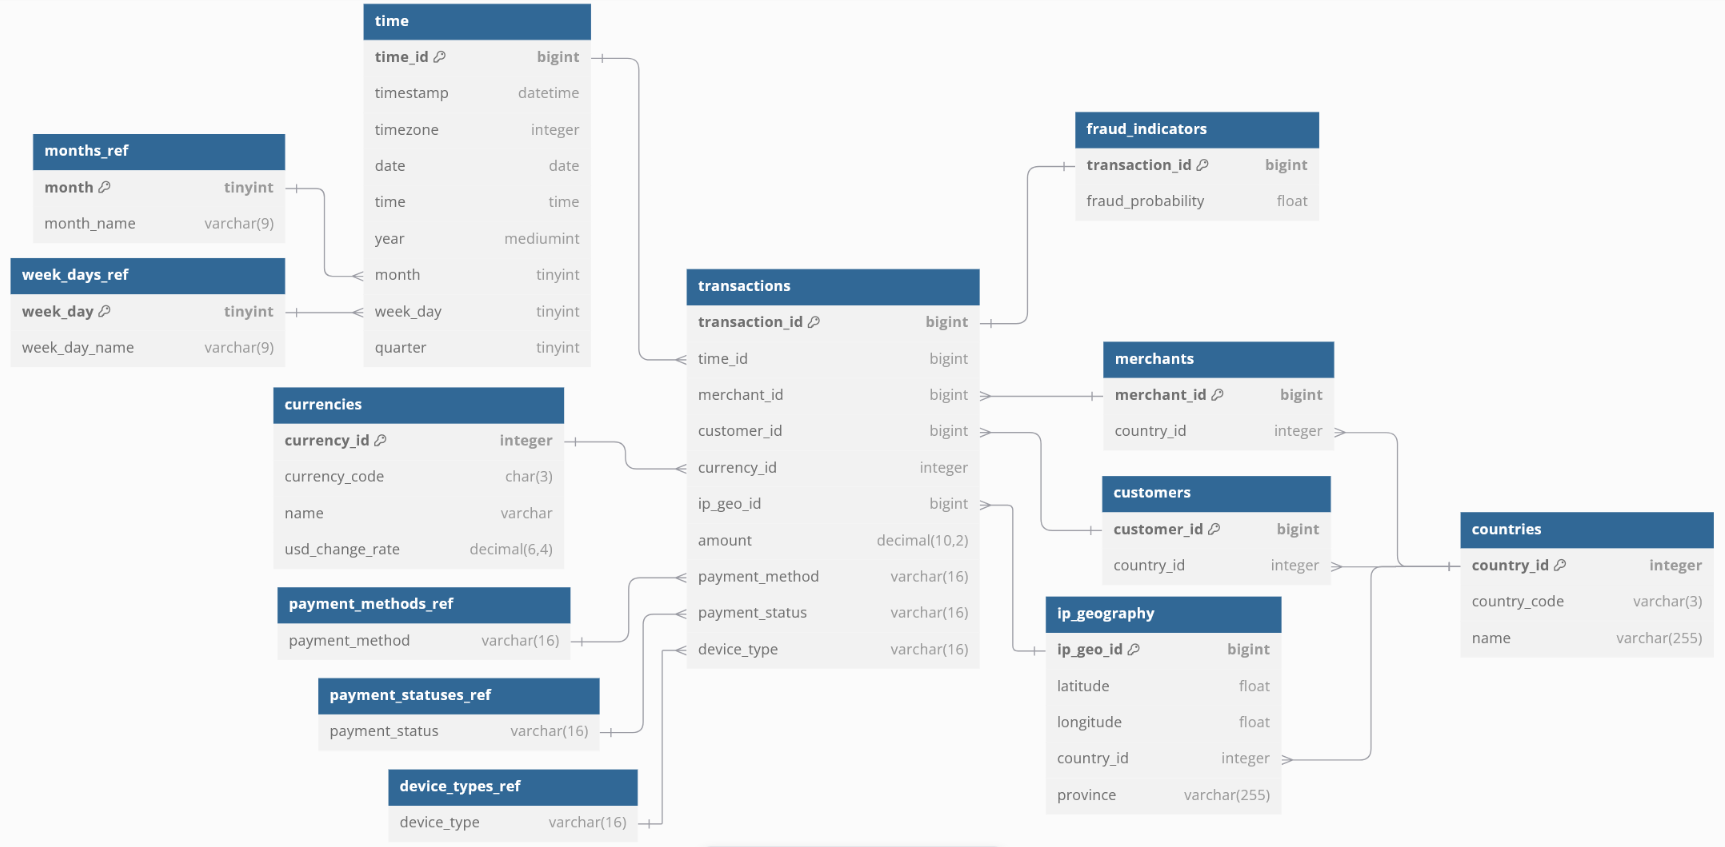
\includegraphics[scale=0.56]{./figures/OLAP}
	\caption{Proposed OLAP database structure.}
	\label{fig:OLAP}
\end{figure}


\begin{table}[ht]
	\centering
	\begin{threeparttable}
		\caption{Data dictionary for the main tables in \code{transactions} OLAP schema.}
		\label{table:OLAP_main}
		\begin{tabularx}{0.99\textwidth}{c c >{\centering\arraybackslash}X >{\centering\arraybackslash}X}
			\toprule
			Field Name & Type & Description & Example  \\
			\midrule
			\multicolumn{4}{c}{\code{transactions} table}\\
			\code{transaction\_id} & \code{bigint} & Unique transaction id & \code{123456789} \\
			\code{merchant\_id} & \code{bigint} & Merchant id & \code{12345} \\
			\code{customer\_id} & \code{bigint} & Customer id & \code{234567} \\
			\code{timestamp} & \code{datetime} & UTC transaction timestamp & \code{2023-11-18T17:43:02.4} \\
			\code{amount} & \code{float} & Transaction amount & \code{43.15} \\
			\code{fee} & \code{float} & Transaction fee & \code{0.53} \\
			\code{currency\_code} & \code{char(3)} & Currency code (ISO 4217) & \code{'GBP'} \\
			\code{payment\_method\_id} & \code{integer} & Payment method id & \code{1} \\
			\code{payment\_status\_id} & \code{integer} & Payment status id & \code{2} \\
			\code{device\_type\_id} & \code{integer} & Device id & \code{3} \\
			\code{ip\_geo\_id} & \code{bigint} & IP geolocation id & \code{123456} \\
			
			\midrule
			\multicolumn{4}{c}{\code{datetimes} table}\\
			\code{timestamp} & \code{datetime} & UTC transaction timestamp & \code{2023-11-18T17:43:02.4} \\
			\code{timezone} & \code{integer} & Timezone offset in minutes & \code{-120} for UTC-02:00 \\
			\code{date} & \code{date} & Transaction date & \code{2023-11-18} \\
			\code{time} & \code{time} & UTC transaction time & \code{17:43:02.4} \\
			\code{year} & \code{mediumint} & Transaction year & \code{2023} \\
			\code{month} & \code{tinyint} & Transaction month & \code{11} \\
			\code{week\_day} & \code{tinyint} & Transaction week day & \code{6} (saturday) \\
			\code{quarter} & \code{tinyint} & Transaction quarter & \code{4} \\
			
			\midrule
			\multicolumn{4}{c}{\code{fraud\_indicators} table}\\
			\code{transaction\_id} & \code{bigint} & Transaction id & \code{123456789} \\
			\code{is\_fraud} & \code{boolean} & Is the transaction a fraud ? & \code{false} \\
			\code{fraud\_score} & \code{float} & Predicted fraud probability & \code{0.12} \\
			
			\midrule
			\multicolumn{4}{c}{\code{ip\_geography} table}\\
			\code{ip\_geo\_id} & \code{bigint} & IP geolocation id & \code{123456} \\
			\code{latitude} & \code{float} & IP-based geolocation lat. & \code{49.6833300} \\
			\code{longitude} & \code{float} & IP-based geolocation long. & \code{10.5333300} \\
			\code{country\_code} & \code{char(2)} & ISO 3166-1 alpha-2 & \code{'DE'} \\
			\code{province} & \code{text} & Province name & \code{'Darmstadt'} \\
			
			\bottomrule
		\end{tabularx}
	\end{threeparttable}
\end{table}


\section*{NoSQL Data Model}

L'entreprise doit aussi gérer des données semi-structurées telles que les fichiers de log, les reçus de transactions ou encore la télémétrie effectuée sur la plateforme de paiement. Les contraintes pour chaque catégorie de données sont diverses et on adoptera une solution basée sur une document-based NoSQL database.

Stripe must handle semi-structured and unstructured data not well-suited to relational models:
\begin{itemize}[itemsep=5pt, parsep=0pt]
	\item \textbf{Telemetry}. Click stream events, user interactions, session data from the payment API.
	\item \textbf{Customer feedback}. Surveys responses, reviews, support transcripts.
	\item \textbf{Log data}. Access and error logs, API usage.
	\item \textbf{Machine learning features}. Generated or derived features used in model inference.
\end{itemize}

We recommend the use of a document-based NoSQL database, such as MongoDB, due to its flexibility in handling nested and heterogeneous data structures.

///The model will follow a domain-oriented, loosely coupled design with a focus on performance and future extensibility.

\begin{figure}
	\centering
	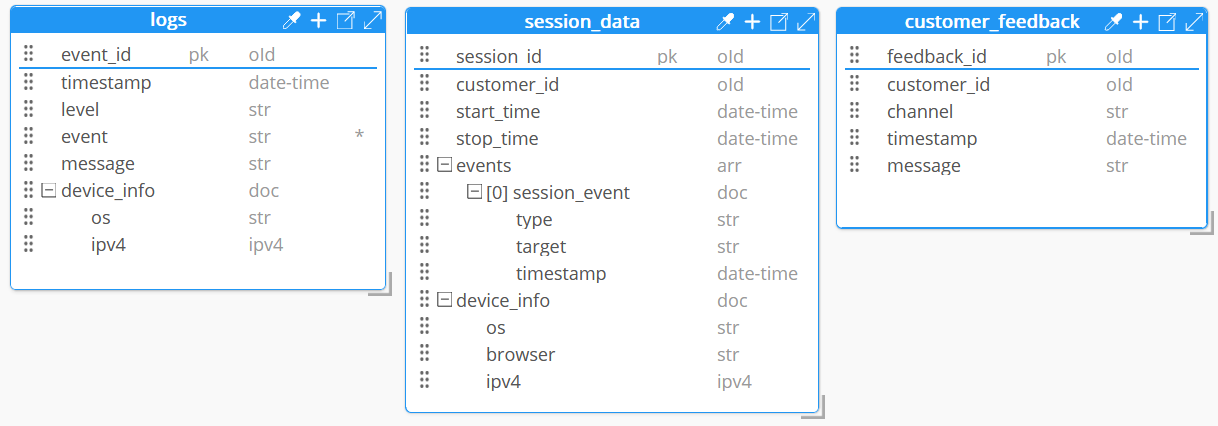
\includegraphics[scale=0.66]{./figures/NoSQL}
	\caption{Illustration of the NoSQL database structure. The schema is made using \href{https://hackolade.com/}{Hackolade} .}
	\label{fig:NoSQL}
\end{figure}


\begin{itemize}
	\item Les informations de session ayant principalement des contraintes de disponibilité associée à des requêtes simples, on s'orientera vers une database de type key-value.
	\item Les fichiers de log sont structurés comme une succession d'évènements. Ceux-ci doivent être stockés de façon à pouvoir alimenter en temps réel des algorithmes de détection d'anomalies, afin d'assurer une réponse rapide en cas d'incident. Il est aussi nécessaire qu'ils soient lisibles par un humain pour une analyse approfondie. On s'orientera donc naturellement vers une document-based NoSQL database pour ce cas d'usage.
	\item Les fichiers non sensibles peuvent être stockés dans un espace approprié (Amazon S3) et indexés par une document-based database qui contiendra aussi les métadonnées.
	\item La télémétrie dans une column database
	\item Les features pour le machine learning peuvent être stockés dans une graph database.
\end{itemize}


\section*{Security and Compliance}

Stripe handles highly sensitive user data, including banking and payment information. Securing this data is critical for two main reasons: first, to comply with international and regional regulations such as GDPR and PCI-DSS; and second, to preserve customer trust. A data breach could result in reputational damage and potential revenue loss.

To minimize the attack surface, sensitive data is isolated within the OLTP system, where it is encrypted both at rest and in transit. Along with the reference database, this system serves as the primary and most secure repository for confidential information.

Some of this data must be made available for analytical purposes, such as detecting financial crimes (e.g., fraud or money laundering). To mitigate risks, the OLAP system only stores anonymized or tokenized derivatives of sensitive fields, such as bank location or institution name, with no direct identifiers. These fields are not encrypted to preserve query performance, but access is strictly controlled through role-based permissions and secure data transfer protocols.

The NoSQL system does not store any sensitive information. Instead, it is used for storing and indexing semi-structured and unstructured data, such as logs or behavioral metadata, none of which poses regulatory risks if properly managed.

Files are handled according to their security classification. Highly sensitive files, like bank receipts, are stored in a dedicated, access-restricted data lake and are indexed only through the OLTP system (not represented in the main architecture diagram). All other files are similarly stored in a general-purpose data lake and indexed via the NoSQL system.

Encrypted backups are created and refreshed at regular intervals to ensure disaster recovery capabilities in the event of a major incident.

Finally, a centralized logging system tracks all server connections, data accesses, and queries. Anomaly detection mechanisms can be integrated to identify and alert on suspicious activities in real time.


\section*{Machine Learning Integration}

Machine learning (ML) plays a critical role in Stripe’s data ecosystem, enabling real-time fraud detection, customer segmentation, and predictive analytics. These use cases require a tightly integrated ML pipeline that supports both batch and real-time processing, and can handle structured as well as unstructured data. The pipeline fulfills three primary functions:
\begin{itemize}
	\item \textbf{Feature extraction and model training}. Features are extracted from OLAP and NoSQL systems, with orchestration handled by tools such as Apache Airflow. Models are trained in cloud-based environments (e.g., AWS EC2) and managed using a model registry (e.g., MLflow) to ensure traceability and version control.
	\item \textbf{Real time inference}. Models are exposed via APIs and queried asynchronously, typically by the OLTP system, to support real-time decision-making (e.g., fraud scoring). Inference responses can trigger automated actions such as alerts or transaction blocks. Models are deployed within a high-availability infrastructure (e.g., Kubernetes) to ensure scalability and low-latency responses under high transaction loads.
	\item \textbf{Batch predictions}. Models are also executed on a scheduled basis to generate insights for use cases like churn prediction or personalization. The resulting predictions are written back to OLAP or NoSQL systems, depending on their usage, and are consumed by recommendation engines or business intelligence tools.
\end{itemize}

Monitoring tools are deployed to track data drift, feature distribution changes, and prediction accuracy over time. Alerts are triggered when drift exceeds defined thresholds. Retraining can be initiated either on a fixed schedule or manually by an operator based on monitoring insights.


\end{document}